\section*{Circuito doble con haz de 3 Conductores}

\begin{figure}[ht!]
\centering
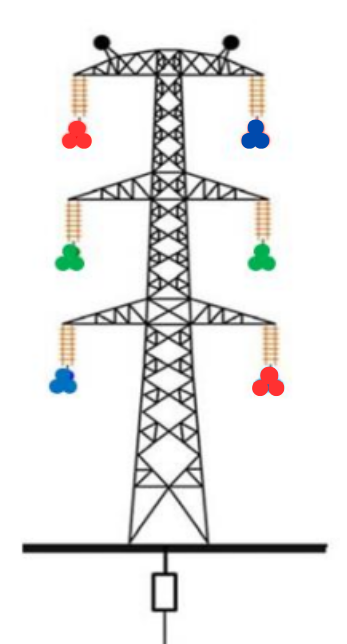
\includegraphics[width=0.48\linewidth]{img/torre3.png}
\caption{Configuración de la torre.}
\label{fig:torre3}
\end{figure}



\begin{figure}[ht!]
\centering
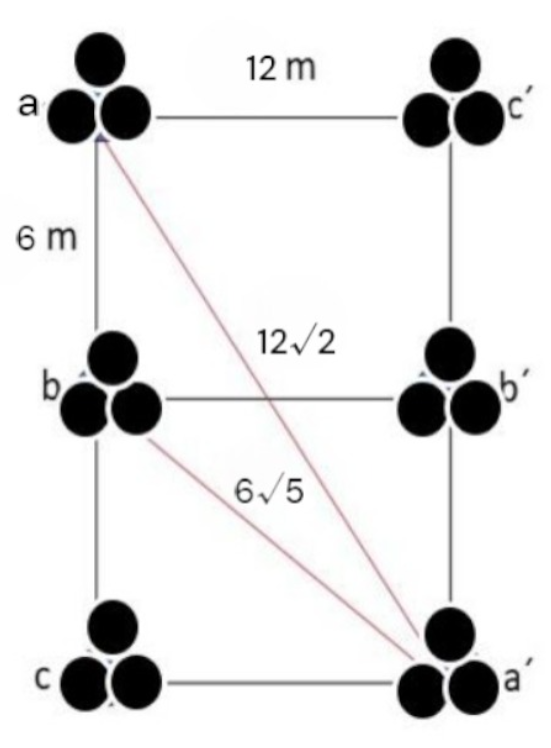
\includegraphics[width=0.48\linewidth]{img/distancia3.png}
\caption{Distancias entre conductores.}
\label{fig:distancia3}
\end{figure}



\textbf{Datos del conductor: Flint 746,4 kcmil}
\begin{itemize}
  \item Longitud línea: $l = 31 \, \text{km}$
  \item Temperatura: $T = 28^\circ$C
  \item $s = 0.4572$ [m]
  \item Radio: $r = 12.58$ [mm]
  \item $f = 60$ [Hz]
  \item RMG = 9.66 [cm]
  \item Resistencia a 75°C: $R_{75} = 0.106 \, \Omega/\text{km}$
  \item $\alpha_0$ aluminio = 0.00438
\end{itemize}

\vspace{0.5cm}

\subsection*{Cálculo de Resistencia equivalente por fase:}

\[
R_{28} = \left( \frac{1 + \alpha_0 \cdot28}{1 + \alpha_0 \cdot 75} \right) \cdot R_{75} = 0.0895488 \, \frac{\Omega}{\text{km}}
\]

\[
R_{\text{eq}} = \frac{l \cdot R_{28}}{6} = \frac{31 \cdot 0.0895488}{6} = 0.4628 \, [\Omega]
\]

\vspace{0.5cm}
\subsection*{Cálculo de Reactancia Inductiva:}

\[
DMG_{AB} = \sqrt[4]{D_{12} \cdot D_{12'} \cdot D_{1'2} \cdot D_{1'2'}} = 8.942 \, [\text{m}]
\]

\[
DMG_{AC} = \sqrt[4]{D_{13} \cdot D_{13'} \cdot D_{1'3} \cdot D_{1'3'}} = 12 \, [\text{m}]
\]

\[
DMG_{BC} = \sqrt[4]{D_{23} \cdot D_{23'} \cdot D_{2'3} \cdot D_{2'3'}} = 8.942 \, [\text{m}]
\]

\[
DMG_{e} = \sqrt[3]{D_{AB} \cdot D_{BC} \cdot D_{CA}} = 9.88524 \, [\text{m}]
\]

\vspace{0.3cm}
\[
RMG_{haz} = \sqrt[3]{RMG \cdot s^2} = 0.2126 \, [\text{m}]
\]

\[
RMG_{a} = \sqrt{RMG_{haz} \cdot D_{11'}} = 1.46457 \, [\text{m}]
\]

\[
RMG_{b} = \sqrt{RMG_{haz} \cdot D_{22'}} = 1.231559 \, [\text{m}]
\]

\[
RMG_{c} = \sqrt{RMG_{haz} \cdot D_{33'}} = 1.46457 \, [\text{m}]
\]

\[
RMG_{e} = \sqrt[3]{RMG_{a} \cdot RMG_{b} \cdot RMG_{c}} = 1.38238 \, [\text{m}]
\]

\vspace{0.3cm}
\[
X_L = 31\cdot 2\pi \cdot f \cdot2\cdot 10^{-4} \cdot \ln\left( \frac{DM_{Ge}}{RMG_e} \right) = 4.54872 \, [\Omega]
\]

\[
z_T = \left[ R_{\text{eq}T} + jX_L \right] = 0,\!4628 + j4,\!5981 \quad [\Omega]
\]

\subsection*{Cálculo de la capacitancia:}

\[
DMG_{e} = \sqrt[3]{D_{AB} \cdot D_{BC} \cdot D_{CA}} = 9.88524 \, [\text{m}]
\]

\[
RMG_{haz} = \sqrt[3]{r \cdot s^2} = \sqrt{0.01258 \cdot 0.4572^2} = 0.138027 \, [\text{m}]
\]

\[
RMG_{a} = \sqrt{RMG_{haz} \cdot D_{11'}} =   1.530489 \, [\text{m}]
\]

\[
RMG_{b} = \sqrt{RMG_{haz} \cdot D_{22'}} = 1.28698 \, [\text{m}]
\]

\[
RMG_{c} = \sqrt{RMG_{haz} \cdot D_{33'}} = 1.530489 \, [\text{m}]
\]

\[
RMG_{e} = \sqrt[3]{RMG_{a} \cdot RMG_{b} \cdot RMG_{c}} = 1.444589 \, [\text{m}]
\]

\[
C_T = \left[ 31 \cdot \left(18 \cdot 10^9 \cdot \ln\left( \frac{DMG_e}{RMG_e} \right) \right)^{-1} \right] = 11.36542 \, [\text{pF}]
\]

\[
Y_T = j\cdot2\pi \cdot f \cdot C_T = j4,\!2846 \times 10^{-9} \quad [\text{S}]
\]

\section*{Parámetros de la línea y receptor:}

\begin{align*}
A &= 1 + \frac{Z_T \cdot Y_T}{2} = 0.9999 + j\,9.911756 \times 10^{-10} \\
B &= Z_T = 0.4628 + j\,4.5981 \quad [\Omega] \\
C &= Y_T \left(1 + \frac{Z_T \cdot Y_T}{4} \right) \\
C &= -2.1241 \times 10^{-18} + j\,4.28466 \times 10^{-9} \quad [S] \\
D &= A = 0.9999 + j\,9.911756 \times 10^{-10}
\end{align*}

\begin{align*}
I_R &= \frac{S}{\sqrt{3} \cdot V_L} \cdot \angle -\cos(\text{fp}) = 1757.15299 \angle -25.844^\circ \quad [A] \\
I_R &= 1757.15299 \angle -25.844^\circ \quad [A] \\
V_R &= \frac{V_L}{\sqrt{3}} \angle 0^\circ = 132.79056 \angle 0^\circ \quad [kV]
\end{align*}

\section*{Parámetros del Generador}

\begin{align*}
V_G &= A \cdot V_R + B \cdot I_R \\
I_G &= B \cdot V_R + D \cdot I_R
\end{align*}

\begin{align*}
V_G &= 137.27837 \angle 2.89^\circ \quad [kV] \\
I_G &= 1757.1574 \angle -25.84478^\circ \quad [A]
\end{align*}

\[
\%RV = \left( \frac{ |V_G| }{ |A| \cdot |V_R| } \right) - 1 = 3{,}33\%
\]
\[
\% \text{Pérdida} = 100*\frac{P_g - P_r}{P_g} = 0{,}6759\%
\]
\[
\% \eta =100* \frac{P_r}{P_g} = 99{,}32\%
\]

\section*{Efecto Corona}

\begin{align*}
m_c &= 0{,}95 \\
m_t &= 1 \\
r &= 400 \quad [\text{m}] \\
T &= 28^\circ \text{C}
\end{align*}

\begin{align*}
h &= 10^{\log_{10}(76) - \frac{y}{18336}} \Rightarrow h = 72.2767 \\
\delta &= \frac{3{,}921 \cdot h}{273 + T} =0.941
\end{align*}

\begin{align*}
U_c &= 84 \cdot m_c \cdot m_t \cdot \delta \cdot \log \left( \frac{DMG}{r} \right) \quad [\text{kV}]
\end{align*}

\begin{align*}
U_{ne} &= 1{,}15 \cdot U_{\text{línea}} \quad [\text{kV}]
\end{align*}

\begin{align*}
U_{ne} < U_c &\Rightarrow 264.5 \leq 273.527 \\
&\text{No se presenta efecto Corona}
\end{align*}